% CREATED BY DAVID FRISK, 2016
\chapter{System Development}

The designed accelerator has a Dataflow architecture, with emphasis on weight data reuse, and it is able to execute a tensor convolution. The basic idea is a computation matrix composed in every entry of processing elements which are able to perform operation between the incoming data and the weights, which have been already loaded for exploiting a data reuse approach.\\
The custom hardware accelerator is not useful as it is. It has to be integrated into a ML-Framework, TensorFlow, which allows to integrate a custom hardware accelerator minimizing the efforts to change the model code and its definitions.

The workflow of the Hardware-Software development is illustrated in the Figure \ref{fig:workflow}.
\begin{figure}[!htbp]
\centering
\captionsetup{justification=centering}
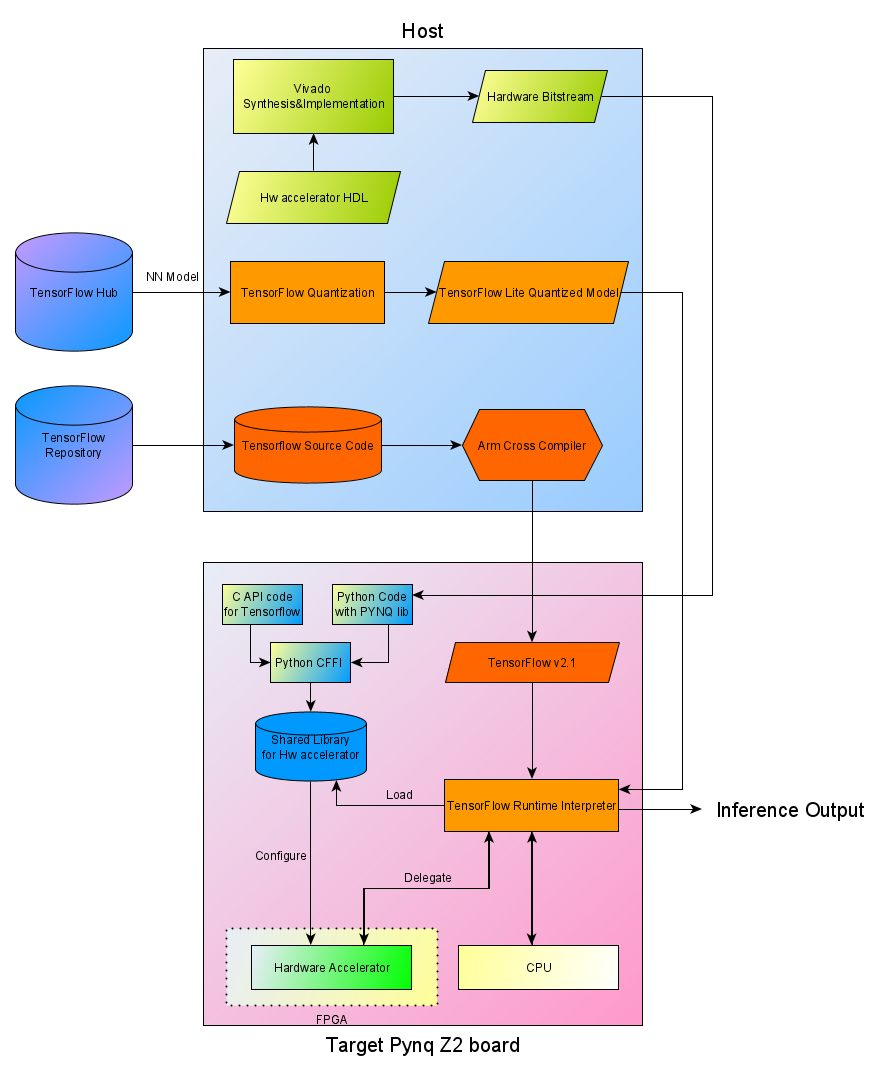
\includegraphics[scale=0.5]{./figure/workflow.png}
\caption{Development workflow}
\label{fig:workflow}
\end{figure}

\section{Software}

The focus of the work is the inference process, pre-trained models are needed and TensorFlow Hub comes in handy for this purpose. It provides already pre-trained Machine Learning models for different domains. Moreover, TensorFlow has the feature of quantizing a post-trained model for different arithmetic precision. In the Fig. \ref{fig:workflow} it can be seen that the quantization process has been done offline.\\
TensorFlow demands as library for the accelerator a C Python-API compatible shared library. In addition, the code for using the accelerator was already written using the PYNQ environment in Python. Therefore, for allowing code reuse and decreasing the development time the Python code has been embedded in the C code (from a TensorFlow example of the delegate library), adding callbacks to Python code.
\section{DTPU, the hardware accelerator}
The hardware accelerator, named \textit{Cogitantium\footnote{Thoughtful}, The Dumb Tensor Processing Unit}, is in charge of carrying out the tensor convolution of the neural network model, exploiting a data-flow architecture on the input data and a data reuse for the weight data.

The work is not focused on developing embedded memories and AXI interfaces, therefore a Xilinx's IP core, which includes all those necessary subcomponents, has been used.
The latter has allowed to completely focus the work on the DTPU core, which has become:
\begin{figure}[H]
\centering
\captionsetup{justification=centering}
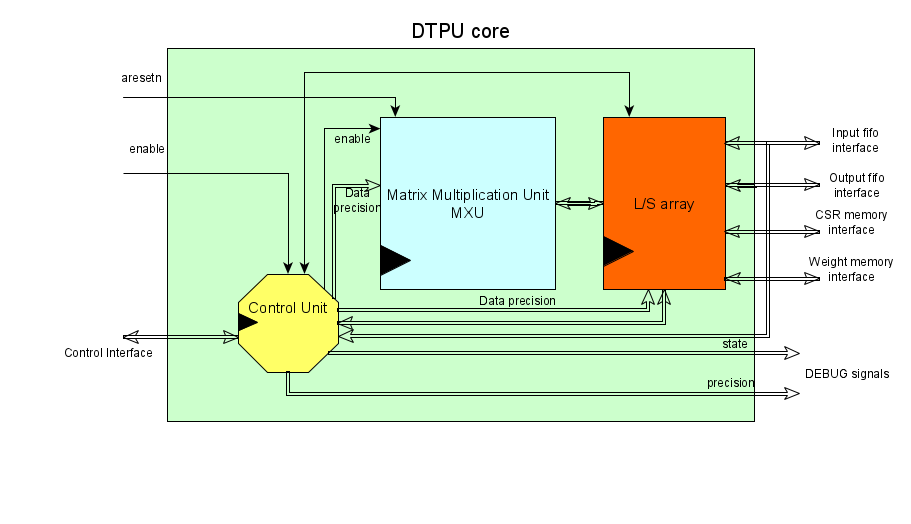
\includegraphics[scale=0.45,angle=0]{./figure/dtpu_core.png}
\caption{RTL view of DTPU core}
\label{fig:dtpucore}
\end{figure}
Where the sub-units:
\begin{itemize}
\item L/S array provides the data for the Matrix Multiplication Unit, especially the weight data are reused across several executions and therefore loaded once. It also provides the correct data to the correct computation units depending on the precision.
\item Control Unit is in charge of handling handshake signals for transferring the ownership of the data (data transferred by the DMA from the Main Memory), load the weights and activation in the respectively units and save the results to the output FIFO. Since it is a Data flow architecture, there is no control flow of the data in the core and this has allowed to keep the Control Unit as simple as possible.
\item Matrix Multiplication Unit (Mxu) is the computation unit of the hardware accelerator, the brawn of the accelerator, a symmetric matrix of MACs with variable precision, where every MAC unit has its own weight value. It executes the tensor convolution for different arithmetic precision.
\end{itemize}